\section{Main Attitude Controller}
\label{sec:mainCont}

\textit{Previously the main attitude controller was treated as a black box. The current and subsequent sections discuss several satellite attitude controllers.}

\subsection{Hybrid Attitude Controller}

Dynamic discontinuous hybrid controller, global asymptotic stability, local exponential stability, state feedback for $\omega$ and $q$. Capable of detumbling. \cite{globalAttController}

There are different ways to describe the rotation of a 3D object. One of them is by using Euler sequences consisting of 3 rotational values. Euler rotation sequences can use combinations of roll, pitch and yaw. There's an inherent problem with Euler rotation, that makes controlling Euler rotation based models an issue, i.e. they are susceptible to singularities. Certain orientations might have an infinite amount of corresponding Euler angles. This can arise when the rotations are made in such a way that some rotation axes align with each other. This issue is commonly known as the gimbal lock. The result of a gimbal lock is that given an attitude, the  cannot be unambiguously deducted, unless extra constraints are introduced.

Quaternion based rotation representation are more appropriate for control. Quaternions are not susceptible to singularities. The only problem with quaternion representation is the so-called double coverage, i.e. rotation by $-\vec{q}$ represents the same rotation as rotation by $-\vec{q}$. This becomes obvious from the rotation equation \ref{eq:doubleCover}.

\begin{equation}
\label{eq:doubleCover}
\vec{q} \vec{v} \vec{q}^{-1} = 	(\vec{-q}) \vec{v} (\vec{-q}^{-1})
\end{equation} 

The attitude control goal can be described as tracking the orientation demand $\vec{q}$. According to \cite{globalAttController}, it is impossible to design a globally stabilizing quaternion based state feedback that is robust to measurement noise. The quaternion-based robust hysteretic feedback controller which is capable of globally asymptotically stabilizing a rigid body is described subsequently, according to \cite{globalAttController}. It can be considered as a more robust extension of classical state feedback controller.


The dynamics of a rigid body is described in equation \ref{eq:dynSimple1}. For clarity of the control method, disturbance torques are emitted from the equation. Since the control system compensates for the gyroscopic term, it is omitted as well from the discussion .

\begin{equation}
\label{eq:dynSimple1}
\underline{I}_s \vec{\dot{\omega}} = \underline{\omega}^\times \underline{I}_s \vec{\omega} + \vec{N_{ctrl}}
\end{equation}

The control goal can be clearly described with rotation matrices. Rotation matrices use 9 variables to describe a rotation, but they have the advantage of being non-ambiguous. The rotation error can be described using equation \ref{eq:rotationError}. 

\begin{equation}
\label{eq:rotationError}
\underline{R}(\vec{q^e}) = \underline{R}(\vec{q^d})^T \underline{R}(\vec{q})
\end{equation}

The goal is to align $\underline{R}(\vec{q})$ with $\underline{R}(\vec{q^d})$ orientation demand. If that demand is satisfied, $\underline{{R}}(\vec{q^e})$ orientation error becomes $\underline{I}$ identity matrix. In quaternion representation, this goal corresponds to having having a unit quaternion with the scalar element being $\pm 1$, according to equation \ref{eq:stabilityQuat}. 

\begin{equation}
\label{eq:stabilityQuat}
\underline{R}(\vec{q^e}) = \underline{R}(\vec{q^e}) = \underline{1} \xrightarrow{equivalent} \vec{q^e}  = \pm	\begin{bmatrix}
0 \\
0 \\
0 \\
1
\end{bmatrix} 	
\end{equation}

Because of the double coverage property of quaternions, stabilizing an attitude, stabilization has to be done on a two equilibrium points corresponding to $\vec{q^e}$ in equation \ref{eq:stabilityQuat}. If a feedback controller is used in the form of $\vec{N_{ctrl}} = f(\vec{q^e})$, $\vec{q^e}$ and $-\vec{q^e}$ might result in different torque demand, even though they both represent the same rotation. Out of the double covering quaternions $[0 0 0 1]^T$ and $-[0 0 0 1]^T$, one might be a stable, the other an unstable equilibrium point. The hybrid controller addresses this issue. According to \cite{globalAttController}, robust and global stabilization on this set is impossible to achieve using non-hybrid discontinuous state feedback in the presence of sensor noise. The paper proposes a hybrid, discontinuous, hysteretic, robust, gloablly asymptotically stabilizing attitude control method instead. A system is considered a hybrid system in the subsequent discussion if the state changes can vary between being continuous or discrete.

The state changes are controlled by the following rules. Controller state storing information about which of the double covering quaternions should be tracked is introduced as $x_c \in  \left\lbrace -1,1 \right\rbrace $. $x_c$ decides which of the two double covering quaternions should be tracked. If $x_c = signum(q_4)$ rule is followed, the controller becomes sensitive to measurement noise. To avoid that, a hysteresis introduced, with an adjustable $\delta  \in (0,1)$ hysteresis threshold parameter. The rule for choosing between discrete or continuous control mode is presented in equation \ref{eq:contDiscont}.

\begin{align}
\label{eq:contDiscont}
C:= \left\lbrace (\vec{q},\vec{\omega},x_c) \in \mathbb{S}^3 \times \mathbb{R}^3 \times \left\lbrace -1,1 \right\rbrace : x_c q_4 \geq -\delta \right\rbrace  \\
\nonumber D:= \left\lbrace (\vec{q},\vec{\omega},x_c) \in \mathbb{S}^3 \times \mathbb{R}^3 \times \left\lbrace -1,1 \right\rbrace : x_cq_4 \leq -\delta \right\rbrace 
\end{align}

If $(\vec{q},\vec{\omega},x_c) \in C$, i.e. the controller is running in continuous mode, the governing equations are according to equation \ref{eq:globalCont}. When $(\vec{q},\vec{\omega},x_c) \in D$, $x_c$ controller state swaps sign instantaneously. Because of the $\delta$ thresholding, two swaps don't happen in infinitesimally small time.  

\begin{align}
	\label{eq:globalCont}
\dot{x}_c = 0, & (\vec{q},\vec{\omega},x_c)  \in C \\
\label{eq:globalDiscont}
x_c^+ = -x_c, & (\vec{q},\vec{\omega},x_c) \in D\
\end{align}

Equation \ref{eq:globalControlInput} describes the generated negative feedback control signal. $K_q$ is the adjustable orientation error gain, $K_e$ is an also adjustable parameter for angular velocity gain.

\begin{equation}
\label{eq:globalControlInput}
\vec{u} = -K_q x_c \vec{q^e}_{1:3} -K_\omega \vec{\omega^e}
\end{equation}

%\begin{align}
%	\label{eq:contDiscont}
%	x_c q_4 \geq -\delta \xrightarrow{}  Continuous \\
%	\nonumber x_c q_4 < -\delta \xrightarrow{}  Discontinuous
%\end{align}


%\[
%\begin{array}{l}
%%\dot{x}_c = 0, (\vec{q},\vec{\omega},x_c) \in C\ \\ 
%x_c^+ = -x_c, (\vec{q},\vec{\omega},x_c) \in D\ \\ 
%%\vec{u} = -c x_c \epsilon -K_\omega \vec{\omega} \\
%%C:= \left\lbrace (\vec{q},\vec{\omega},x_c) \in \mathbb{S}^3 \times \mathbb{R}^3 \times \left\lbrace -1,1 \right\rbrace : x_c\eta \geq -\delta \right\rbrace  \\
%%
%%D:= \left\lbrace (\vec{q},\vec{\omega},x_c) \in \mathbb{S}^3 \times \mathbb{R}^3 \times \left\lbrace -1,1 \right\rbrace : x_c\eta \leq -\delta \right\rbrace 
%\end{array}
%\]

\subsubsection{Detumbling}

After a satellite is ejected from its rocket, it might be rotating quite fast. The first task of the satellite attitude controller is detumbling the satellite, preparing for normal operation. The hybrid attitude controller is capable of doing that. This means that the hybrid attitude controller is a good nominee for being the attitude controller for every operation mode. A simulation was made where the satellite's initial angular velocity is unrealistically high, while the control goal is stabilizing the satellite to point at the nadir. Actuator saturation is omitted in order to present the dynamics of the control law more clearly. Figures \ref{fig:detumbling} and \ref{fig:detumblingomega} present the torque demand and the angular velocity during detumbling. At 4 seconds, the input quaternion is negated in order to present the controller handling the double coverage of the quaternion. Figure \ref{fig:detumblingVar} presents $x_c$ during the detumbling maneuver.

%At the current level of analysis, motor and magnetorquer models are omitted, it is assumed that the actuators satisfy the attitude controller's torque demand. Simulation results with actuator models are presented in subsequent chapters.


\begin{figure}[H]
	\centering
%	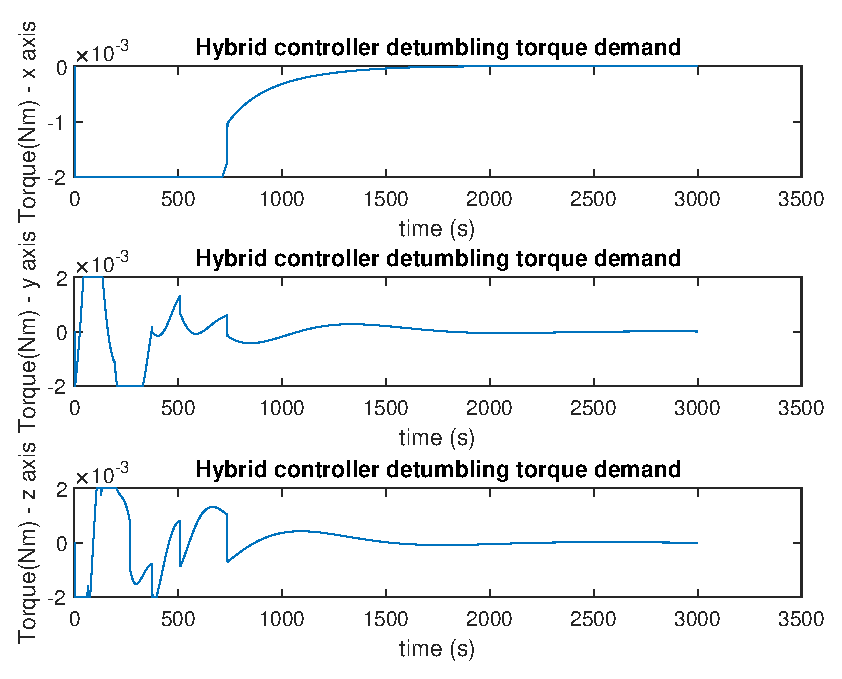
\includegraphics[width=0.7\linewidth]{figures/detumbling}
	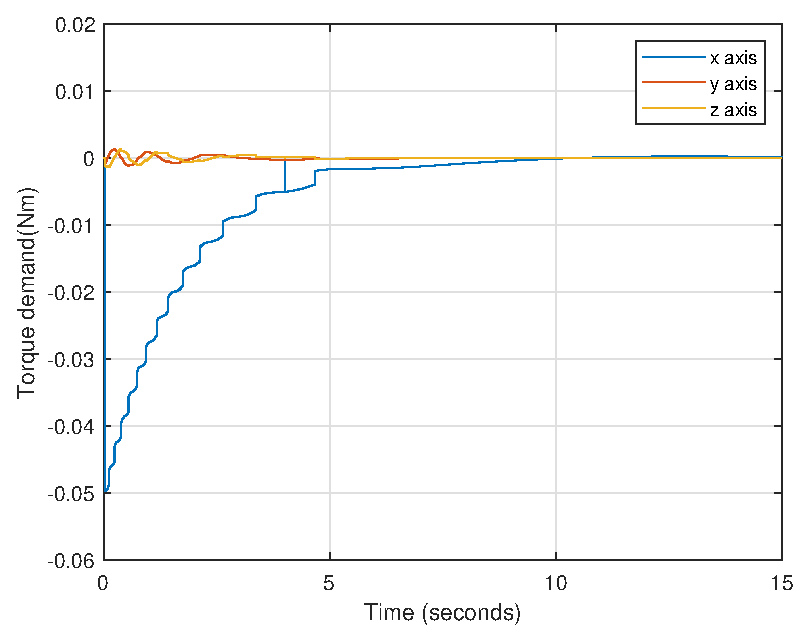
\includegraphics[width=0.9\linewidth]{figures/hybridtorque}
	\caption{Hybrid controller detumbling torque demand}
	\label{fig:detumbling}
\end{figure}

\begin{figure}[H]
	\centering
%	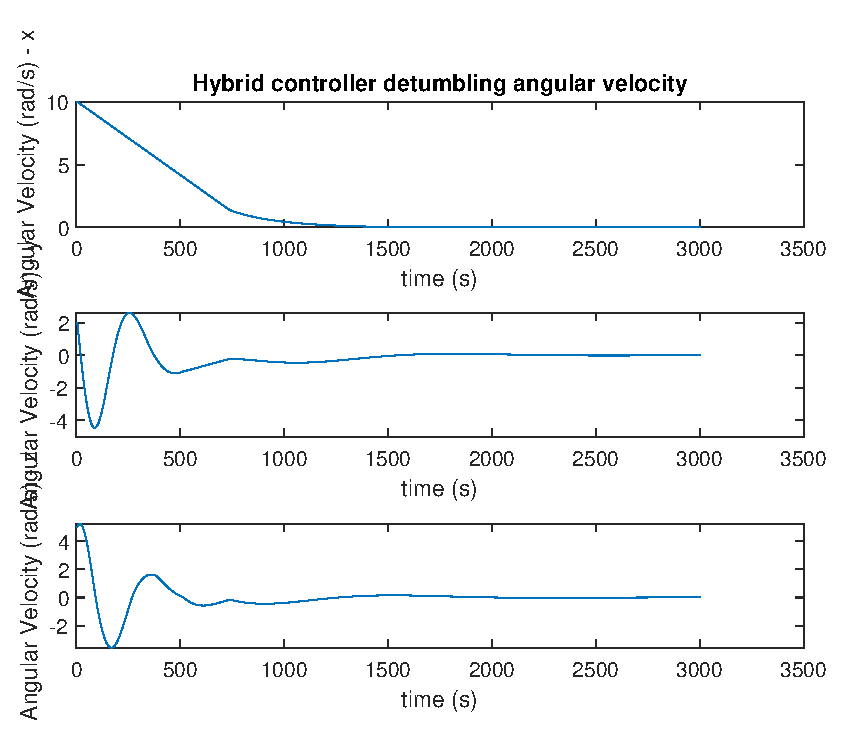
\includegraphics[width=0.7\linewidth]{figures/detumbling3}
	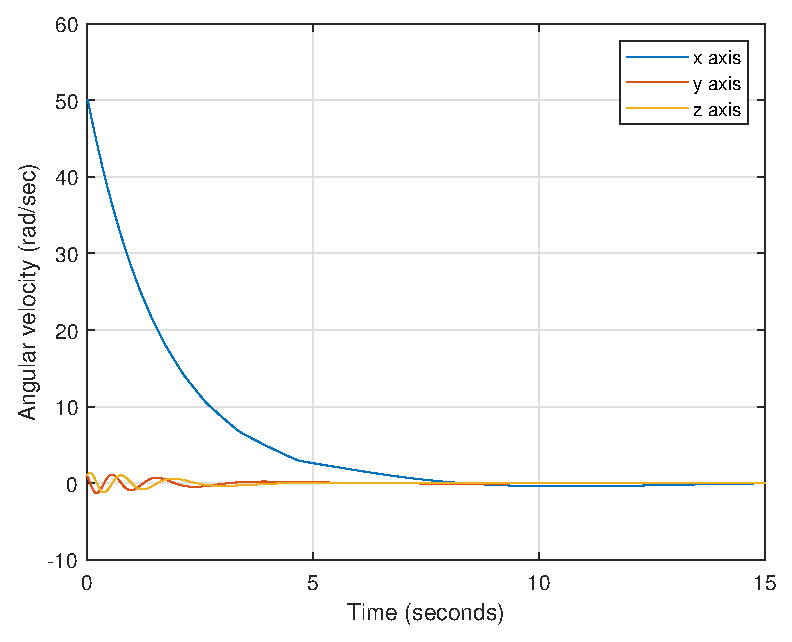
\includegraphics[width=0.7\linewidth]{figures/hybridomega}
	\caption{Satellite angular velocity during detumbling maneuver using the hybrid controller}
	\label{fig:detumblingomega}
\end{figure}

\begin{figure}[H]
	\centering
	%	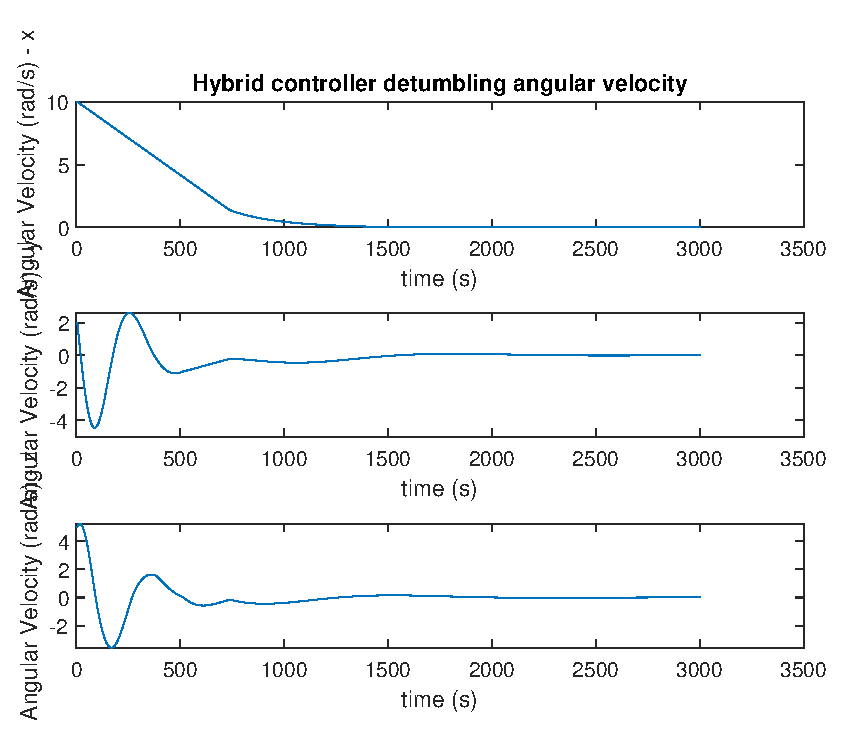
\includegraphics[width=0.7\linewidth]{figures/detumbling3}
	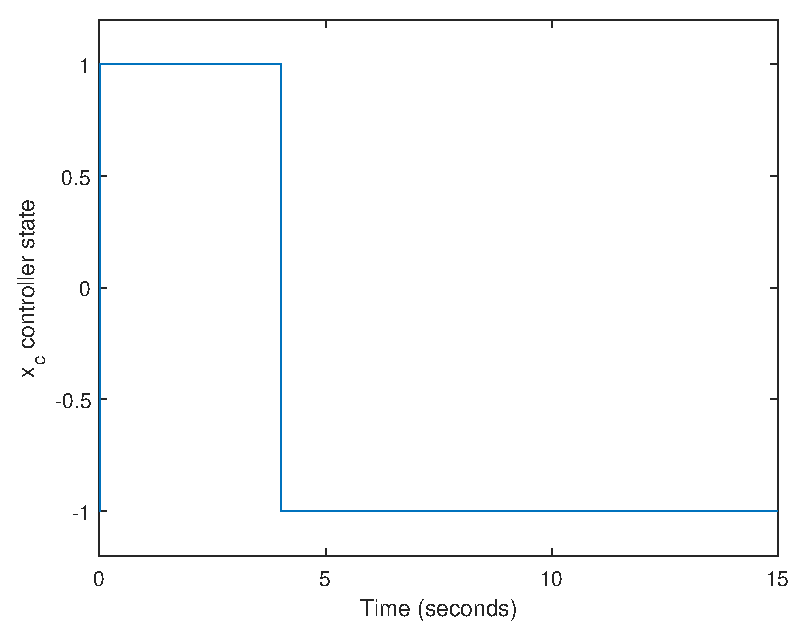
\includegraphics[width=0.4\linewidth]{figures/xc}
	\caption{$x_c$ controller state during detumbling maneuver using the hybrid controller. The quaternion error is negated at 4 seconds.}
	\label{fig:detumblingVar}
\end{figure}


